% 公立はこだて未来大学 卒業論文 テンプレート ver1.50
% (c) Junichi Akita (akita@fun.ac.jp), 2003.10.31
% update by N.T.,  2004.11.10
%
\documentclass{funthesis}
%¥documentclass[english]{funthesis} % use [english] option for English style

\usepackage{graphicx} % 図(EPS形式)を本文中で読み込む場合はこれを宣言
\usepackage{url}

% この部分に,タイトル・氏名などを書く.
% タイトルなどの定義の始まり
\jtitle{知識ベース型推薦を用いたフードツーリズム支援システムの構築}% 論文の和文タイトル
%
\etitle{Development of a Food Tourism Support System Using Knowledge-based Recommendation}% 論文の英文タイトル
%
\htitle{Development of a Food Tourism Support System Using Knowledge-based Recommendation}   % ヘッダー用の論文の短縮英文タイトル
%     必ず1行に収まるように英文タイトルを短縮する.
%
\jauthor{三好 良弥}     % 氏名(日本語)
\eauthor{Ryoya Miyoshi}   % 氏名(英語)
\jaffiliciation{情報アーキテクチャ学科} % 所属学科名(日本語)
\eaffiliciation{Department of Media Architecture} % 所属学科名(英語)
\studentnumber{1014127}   % 学籍番号
\jadvisor{奥野 拓}    % 正指導教員名(日本語)
%¥jcoadvisor{} % 副指導教員(日本語)がいる場合は
                        % コメントアウトし名前を書く
                        % 副指導教員がいない場合は,ここは削除しても可
\eadvisor{Taku OKUNO}  % 正指導教員名(英語)
%¥ecoadvisor{}   % 副指導教員(英語)がいる場合は
                         % コメントアウトし名前を書く
                         % 副指導教員がいない場合は,ここは削除しても可
\jdate{平成30年01月29日}    % 論文提出日   (日本語)
\edate{January 29, 2018}     % 論文提出年月 (英語)
% タイトルなどの定義の終わり

\begin{document}

%--------------------------------------------------------------------
\maketitle       % タイトルページを作成

%--------------------------------------------------------------------
% 英文概要(250語程度)
\begin{eabstract}
hoge hoge hoge hoge hoge hoge hoge hoge hoge hoge hoge hoge hoge hoge hoge hoge hoge hoge hoge hoge hoge hoge hoge hoge hoge hoge hoge hoge hoge hoge hoge hoge hoge hoge hoge hoge hoge hoge hoge hoge hoge hoge hoge hoge hoge hoge hoge hoge hoge hoge hoge hoge hoge hoge hoge hoge hoge hoge hoge hoge hoge hoge hoge hoge hoge hoge hoge hoge hoge hoge hoge hoge hoge hoge hoge hoge hoge hoge hoge hoge hoge hoge hoge hoge hoge hoge hoge.
\end{eabstract}

% 英文キーワード(5個程度をコンマ(,)で区切って羅列する)
\begin{ekeyword}
Kowledge-based Recommender System
\end{ekeyword}

%--------------------------------------------------------------------
% 和文概要(300字程度)
\begin{jabstract}
近年,地域らしい料理を食べることを目的とした旅であるフードツーリズムが盛んである.しかし,観光客の嗜好によって地域らしい料理の判断基準が異なるため,従来のグルメサイトでは地域らしい料理を探すことが困難である.この問題を解決するために,観光客の嗜好を考慮した地域らしい料理推薦システムを提案する.グルメサイトからWebスクレイピングを行い抽出した飲食店及び料理の情報を用いてデータベースを構築し,観光客の嗜好にあった地域らしい料理の推薦を行う.推薦手法として,「評価が高い商品」や「1000円以下の商品」などユーザが商品に求める具体的な条件がある場合に有効な知識ベース型推薦を用いることで,嗜好にあった料理の推薦を可能にする.

\end{jabstract}

% 和文キーワード(5個程度をコンマ(,)で区切って羅列する)
\begin{jkeyword}
知識ベース型推薦
\end{jkeyword}

%--------------------------------------------------------------------
\tableofcontents % 目次を作成



%--------------------------------------------------------------------
% ¥includegraphics[width=??cm]{hoge.eps} % 図(EPS形式)を読み込む場合


%--------------------------------------------------------------------
\chapter{序論} 

\section{背景}
近年,ニューツーリズムの振興[1] により,地域らしい料理が重要な観光資源となっている.こうした,地域らしい料理を食べることを目的とした旅のことをフードツーリズムと呼ぶ.日本フードツーリズム協会[2] は,フードツーリズムを,地域ならではの料理・食文化をその地域で楽しむための旅と定義している.また,フードツーリズムには地域らしい料理・食文化,それを引き立てる体験,場所,人の4 つの要素があると定義している.

じゃらんが実施したアンケート[3] では,観光客が観光地を選んだ理由のひとつとして「地域らしい料理・特産品に興味があったから」と回答した人が41.6\%であった.このことから,観光客は地域らしい料理を旅行の際に重要視していることがわかる.

観光客がフードツーリズムの重要な要素である地域らしい料理を探す方法の一つとしてグルメサイトを用いて検索する方法がある.しかし,観光客によって地域らしい料理に求める条件が異なるため,観光客が期待する料理を探すことは容易ではない.

\section{研究目的}  
本研究では観光客の嗜好や状況を考慮した地域らしい料理の推薦を行うことで観光客の満足度向上を目指す.そこで,本研究では知識ベース型推薦を用いた地域らしい料理推薦システムを提案する.

\section{本論文の構成}
本論文は全6章で構成されている.第1章では,本研究の背景および研究目的について述べた.第2章では,関連技術について述べる.第3章では,関連研究について述べる.第4章では,本研究で提案する地域らしい料理推薦システムの構築について述べる.第5章では,実験方法および実験の結果,結果から得られた考察について述べる.最後に第6章では,本研究のまとめと今後の展望を述べる.

%--------------------------------------------------------------------
\chapter{関連技術}

\section{情報推薦手法}
情報推薦に用いられる代表的な手法は,協調ベース型推薦,内容ベース型推薦,知識ベース型推薦がある.それぞれの手法について以下で述べる.

\subsection{協調ベース型推薦}
協調ベース型推薦とは....

\subsection{内容ベース型推薦}
内容ベース型推薦とは....

\subsection{知識ベース型推薦}
知識ベース型推薦とは....

\section{本研究で用いる手法}

%--------------------------------------------------------------------
\chapter{関連研究}%嗜好を用いた推薦について記述

%--------------------------------------------------------------------
\chapter{提案手法}

\section{使用するデータの収集}
本研究では,複数のグルメサイトからWebスクレイピングにより函館市の料理および飲食店の情報を収集した.収集した情報は表1,2の各属性と店舗の口コミである.収集した情報をもとに推薦の際に使用するデータベースを構築した.
収集した情報は,飲食店の情報が2,206件,料理の情報が9,866件,口コミの情報が14,974件である.

\section{推薦アルゴリズム}
本研究で用いた知識ベース型推薦のアルゴリズムを図 1に示す.以下に顧客要求と製品制約,効用にもとづくソートについて記述する.

\begin{figure}
  \begin{center}
    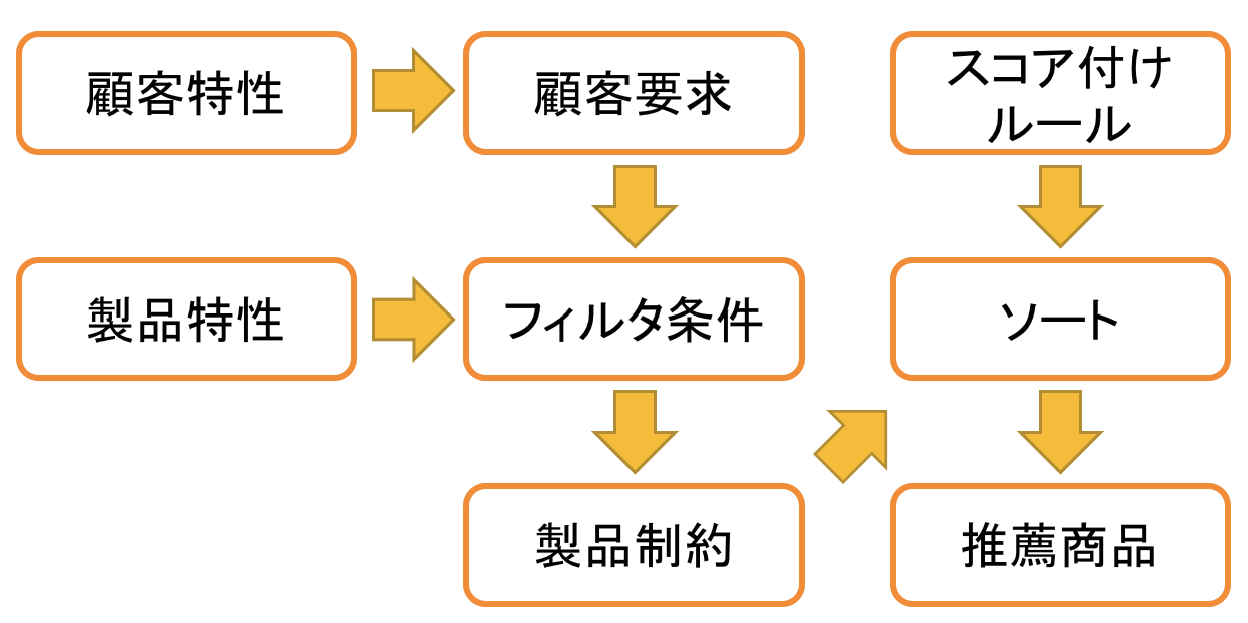
\includegraphics[clip,width=8.3cm]{model.eps}
    \caption{知識ベース型推薦のアルゴリズム}
  \end{center}
\end{figure}

\subsection{顧客要求}
知識ベース型推薦では,顧客特性をもとに顧客要求を設定する.顧客特性とは,ユーザが商品を選ぶ際に使用する項目の集合である.本研究では顧客特性に,予算,ジャンルを使用する.顧客要求とは,ユーザがどのような顧客特性を持っているかをまとめた集合である.本研究での顧客要求の例として「予算は1000円,ジャンルは洋食の料理が食べたい」が挙げられる.

\subsection{製品制約}
知識ベース型推薦では,顧客要求と製品特性をもとにフィルタ条件を用いて,ユーザが満たして欲しい条件を設定する.本研究において製品特性とは,料理及び店舗が持つすべての属性である.本研究で定義した製品特性の例を表1,2に示す.
フィルタ条件とは,顧客要求と製品特性との関係を定義したものである.例えば,顧客要求として「予算が1000円」と入力された場合,「価格」が1000円以下の料理に絞り込む.

\begin{table}
  \begin{center}
  \scriptsize
    \caption{製品特性の例(料理)}
    \begin{tabular}{p{3.6cm}|p{3.6cm}} 
    \hline
属性 & 値 \\ \hline\hline
      料理id & 149\\ \hline
      料理名 & 塩ラーメン \\ \hline
      価格(円) & 580 \\ \hline  \end{tabular}
  \end{center}
  \end{table}
  
\begin{table}
  \begin{center}
  \scriptsize
    \caption{製品特性の例(店舗)}
   \begin{tabular}{p{3.6cm}|p{3.6cm}} 
    \hline
属性 & 値 \\ \hline\hline
      店舗id & 6\\ \hline
      店名 & 星龍軒 \\ \hline
      住所 &  北海道函館市若松町7-3\\ \hline
      オープン年(年)& 1951 \\ \hline
      ジャンル & ラーメン、餃子、中華料理 \\ \hline
      緯度 & 41.771268 \\ \hline
      経度 & 140.7264993 \\ \hline
  \end{tabular}
  \end{center}
\end{table}

\subsection{効用にもとづくソート}
知識ベース型推薦では,効用に基づくソートを行う.本研究では,「地域発祥の料理」,「古くからある店舗」,「地域でしか食べられない料理」,「人気のある料理」の4項目の観点でユーザの効用を求め,ソートを行う.効用は式(1)で求めることができる.
\begin{equation}
効用(p)=\sum_{j=1}^{n} 関心度(j)×貢献度(p,j) 
\end{equation}

{\it p}は料理,{\it j}は観点を表す.関心度とはある観点においてどれほど商品に関心があるのかを表した度合いである.本研究では関心度をユーザに入力してもらう.貢献度とは商品がある観点にどれだけ貢献しているかを表した度合いである.本研究ではスコア付けルールを用いて貢献度を設定する.スコア付けルールとは料理および店舗の属性をもとに本研究で定義した観点を数値化するものである.本研究で定義したスコア付けルールを表 3に示す.

\begin{table}
  \begin{center}
  \scriptsize
    \caption{貢献度のスコア付けルール}
   \begin{tabular}{p{3.4cm}|p{3.9cm}} 
    \hline
観点 & 数値の基準 \\ \hline\hline
      地域発祥の料理 &  料理の発祥した場所が函館市に近いほど,貢献度が大きい\\ \hline
      古くからある店舗 & 店の開店日が古いほど,貢献度が大きい\\ \hline
      地域でしか食べられない料理 & 首都圏で取り扱っている店舗が少ないほど,貢献度が大きい\\ \hline
      人気のある料理 & お店の人気と料理の人気があるほど,貢献度が大きい \\ \hline
  \end{tabular}
  \end{center}
\end{table}

\section{システムの実装}

%--------------------------------------------------------------------
\chapter{実験}

%--------------------------------------------------------------------
\chapter{結論}

\section{まとめ}

\section{今後の展望}

\chapter *{謝辞}



%--------------------------------------------------------------------
% 参考文献
\begin{thebibliography}{7}
\end{thebibliography}

% 表目次の表示
\listoftables

% 図目次の表示
\listoffigures

\end{document}
